\documentclass{article}
\usepackage[utf8]{inputenc}
\usepackage{graphicx}
\usepackage{booktabs}
\usepackage{amsmath, amsthm, amssymb, bm}
\usepackage{tikz, pgfplots}
\usepackage{float}
\usepackage[hidelinks]{hyperref}

\title{Verifying Central Limit Theorem}

\author{Dishank (AI20BTECH11011),\\ Chirag (AI20BTECH11006),\\ Vishwanath (MA20BTECH11010),\\ Savarana Datta Reddy (AI20BTECH11008)}
\date{April 2022}


\begin{document}
\maketitle

\section{Introduction}
Central Limit Theorem states that normalised sum of independent and identically distributed random variables tends towards a normal distribution, irrespective of the distribution of random variables.
\begin{align}
    Z = \lim_{n \to \infty} \left(\frac{\bar{X}_n-\mu}{\frac{\sigma}{\sqrt{n}}}\right) \label{eq:CLT}
\end{align}
In this project, we propose to verify the correctness of Central Limit Theorem by running simulations beginning with a variety of distributions covered in the course.

\section{Central Limit Theorem and empirical approximation}
While equation \eqref{eq:CLT} suggests that $n$ should be a very large number. In practice, we tend to use the theorem for $n>30$. 
\subsection{Assumptions}
\begin{itemize}
\item  The samples drawn are independent.
\item  The sample size is sufficiently large
\item  The mean and variance of the sampling distribution are finite
\end{itemize}
\subsection{Proof}
Let $X_1,X_2,\dots,X_n,\dots$ be i.i.d random variables with mean $\mu$ and variance $\sigma^2$.
The sum $X_1+X_2+X_3+\dots+X_n,$ has mean = $n\mu$ and variance $n\sigma^2$.

Now consider the random variable 
\begin{equation}
    Z = \frac{X_1+X_2+X_3+\dots+X_n - n\mu}{\sqrt{n\sigma^2}}
\end{equation}
which is equivalent to 
\begin{equation}
    Z = \sum_{i=1}^n \frac{Y_i}{\sqrt{n}}
\end{equation}
where,
\begin{equation}
    Y_i = \frac{X_i-\mu}{\sigma}\label{a}
\end{equation}
Each with mean = 0 and variance = 1.

Since $Y_i$'s are all identically distributed the characteristic equation of $Z$ is given as.
\begin{equation}
    \phi_{Z}(t) =\displaystyle \prod_{i=1}^n\phi_{Y_n}\left(\frac{t}{\sqrt{n}}\right) = \left[\phi_{Y_1}\left(\frac{t}{\sqrt{n}}\right)\right]^n
\end{equation}
The characteristic equation of $Y_1$ is given
\begin{equation}
    \phi_{Y_1}\left(\frac{t}{\sqrt{n}}\right) = \left(1-\frac{t^2}{2n} + o\left(\frac{t^2}{n}\right)\right), \;\; \left(\frac{t}{\sqrt{n}}\right)\to 0 \label{b}
\end{equation}
o is the little o notation.

Now the Characteristic equation of $Z$ in equation \eqref{a} is 
\begin{equation}
    \phi_{Z}(t) = \left( 1-\frac{t^2}{2n} + o\left(\frac{t^2}{n}\right) \right)^n
\end{equation}
We know that 
$$\lim_{n\to\infty} \left(1+\frac{x}{n}\right)^n = e^x$$
When we apply $\lim_{n\to\infty}$ the equation \eqref{b} will change into 
\begin{equation}
    \lim_{n\to\infty}\phi_{Z}(t) =\lim_{n\to\infty}\left( 1-\frac{t^2}{2n} + o\left(\frac{t^2}{n}\right) \right)^n =  e^{\frac{-1}{2}t^2}
\end{equation}
As all the higher terms will disappear as n goes to higher values.
So, The R.H.S will be equal to Characteristic equation of $\mathcal{N}(0,1)$.
Therefore as $n\to\infty$ the distribution $Z$ will approach $\mathcal{N}(0,1)$.
i.e. $\frac{\sqrt{n}}{\sigma}(\Bar{X}_n - \mu) $ converges to the Normal distribution $\mathcal{N}(0,1)$.
Hence proved.

\section{Shapiro-Wilk Test}
The Shapiro–Wilk test is used to determine whether a sample $x_{1},..., x_{n}$ was drawn from a normally distributed population.\\
The test statistic(W):
\begin{align}
    W=\frac{\left(\displaystyle\sum_{i=1}^{n}a_{i}x_{(i)}\right)^{2}}{\displaystyle\sum_{i=1}^{n}(x_{i}-\bar{x})^{2}}
\end{align}
where
\begin{itemize}
    \item $x_{(i)}$ is $i^{th}$ order statistic i.e, $i^{th}$ smallest element in the sample.
    \item $\bar{x}$ is mean of the sample($x_{1},\dots,x_{n}$). 
    \item $(a_{1},a_{2},\dots,a_{n})=\frac{m^{\top}V^{-1}}{C}$ where $C=||V^{-1}m||$.
    \item $\underbar{m}$ is composed of the expected values of the order statistics of independent and identically distributed random variables drawn from a typical normal distribution.
    \item $\mathbf{V}$ is the covariance matrix of those normal order statistics
\end{itemize}

\subsection{Alternative way of estimating $W$}
\noindent The Shapiro-Wilk statistic can be calculated using following steps:
   \begin{itemize}
           \item Order the data from the least to greatest. $x_{j}$ denotes the ($j^{th}$) order statistic i.e, $j^{th}$ smallest element in the set.
           \item We calculate value $X_{(n-i+1)}-X_{(i)}$ for i in range [0,$\lceil{n/2}\rceil$]
           \item Get the Shapiro-Wilk coefficients($a_{in}$) from the \href{https://github.com/cmaspi/verifying_CLT/tree/main/latex/report/images/coefficients}{table} and calculate the value of b.
            \begin{align}
              b=\sum_{i} b_{i} = \sum_{i=1}^{\lceil{n/2}\rceil} \left(X_{(n-i+1)}-X_{(i)}\right) a_{in} 
            \end{align}
            \item Calculate standard deviation($s$) of the data set to estimate the Shapiro-Wilk statistic ($W$)
            \begin{align}
                W = \frac{b^{2}}{s^{2}(n-1)}
            \end{align}
       \end{itemize}
       This estimate of W is close enough to the original one for $n\leq50$.

\subsection{Interpretation}
This test assumes that the population is regularly distributed. If the p value is smaller than the selected alpha level, the null hypothesis is rejected, and evidence that the data being tested are not normally distributed is found. The null hypothesis, on the other hand, cannot be rejected if the p value exceeds the set alpha threshold. Generally we consider alpha threshold as 0.05.
\begin{itemize}
    \item \textbf{If p $\leq$ 0.05}: then the null hypothesis can be rejected (i.e. the variable is NOT normally distributed).
    \item \textbf{If p $>$ 0.05}: then the null hypothesis cannot be rejected (i.e. the variable \textbf{MAY BE} normally distributed).
\end{itemize}
You can find the table for minimum W value required for particular  n and p values
\href{https://github.com/cmaspi/verifying_CLT/tree/main/latex/report/images/p_value}{here}.\\

\subsection{Examples}
\textbf{Example - 1}\\
The following data represents the concentration of nickle in solid waste,\begin{align*} 58.8,19,39,3.1,1,81.5,151,942,262,
    331,\\27,85.6,56,14,21.4,10,8.7,64.4,578,637 \end{align*}
    \begin{itemize}
 
        \item Arrange in ascending order X=[1, 3.1, 8.7, 10, 14, 19, 21.4, 27, 39, 56, 58.8, 64.4, 81.5, 85.6, 151, 262, 331, 578, 637, 942]
        \item Difference Matrix = $[ 941,633.9,569.3,321,248,132,64.2,54.5,25.4,2.8]$
        \item Shapiro-Wilk coefficients for n=20 is  
        [0.4734, 0.3211, 0.2565, 0.2085, 0.1686, 0.1334, 0.1013, 0.0711, 0.0422, 0.0140]
        \item b value is $=(941)(0.4734)+(633)(0.3211)+\dots = 932.8$
        \item Standard Deviation of the data set $s=259.72$
        \item The value of $W=\frac{b^{2}}{s^{2}(n-1)}=0.679$. The minimum value of w needed to have p-value of at least 0.05 is 0.905 (for n=20). As the observed $W<0.905$ we can conclude that the given data set is not normally distributed.
    \end{itemize}

\noindent \textbf{Example - 2}\\
Consider the following data
$$20,38,40,45,50,63,70,75,79,86$$
\begin{itemize}
    \item Ascending order = $20,38,40,45,50,63,70,75,79,86$
    \item Difference Vector = $66,41,35,25,13$
    \item Shapiro-Wilk coefficients for n=10 are $0.5739,0.3219,0.2141,0.1224,0.0339$
    \item The value of b = 62.095
    \item The value of $W=0.959$. The minimum value of w needed to have p-value of at least 0.05 is 0.869 (for n=10). As the observed $W>0.869$ we can say that the data set behaves like a normal distribution. 
\end{itemize}

\noindent You can find the python codes implementing the above examples 
\href{https://github.com/cmaspi/verifying_CLT/blob/main/codes/examples.ipynb}{here}.

\subsection{Why it works?}
The Shapiro-Wilk is more powerful because it also takes into account the co variances between the order statistics, producing a best linear estimator of $\sigma$ from the Q-Q plot, which is then scaled by s. When the distribution is far from normal, the ratio isn't close to 1.



\section{Hypothesis}
The hypothesis can be framed as follows
\begin{align}
    & H_A\text{ : The empirical approximation of the CLT does not hold} \nonumber\\
    & H_0\text{ : The empirical approximation of the CLT holds}\nonumber
\end{align}
The significance level $\alpha$ is subject to the method of normality testing. For our case, the Shapiro-Wilk test suggests using a significance level of $0.05$. 
% This means that if we obtain a p-value less than alpha, we reject the null hypothesis. Otherwise, we fail to reject the null hypothesis.

\section{Procedure}
We have chosen 4 sampling distributions. For each distribution, we generated 1000 batches of sizes 10, 30, 50 and 100 samples from the sampling distribution. We find the sample mean of each batch and call it $\bar{X}$. From Central Limit Theorem, we know
\begin{align}
    \bar{X} \sim \mathcal{N}\left(\mu, \frac{\sigma^2}{n}\right)
\end{align}
To verify the claim, we perform normality tests, which can be classified into two parts
\begin{enumerate}
    \item Graphical Methods
    \begin{itemize}
        \item Histogram
    \end{itemize}
    \item{Frequentist tests}
    \begin{itemize}
        \item Shapiro-wilk test
    \end{itemize}
\end{enumerate}

\subsection{Distributions used}
\begin{enumerate}
    \item \textbf{Standard Normal}: The pdf of standard normal distribution is given by:
    $$f_X(x) = \dfrac{1}{\sqrt{(2\pi)}}exp\left(-\dfrac{x^2}{2}\right)$$
    The mean is 0 and standard deviation is 1. Figure \ref{normal_pdf} shows the PDF of standard normal distribution.
    \begin{figure}[H]
        \centering
        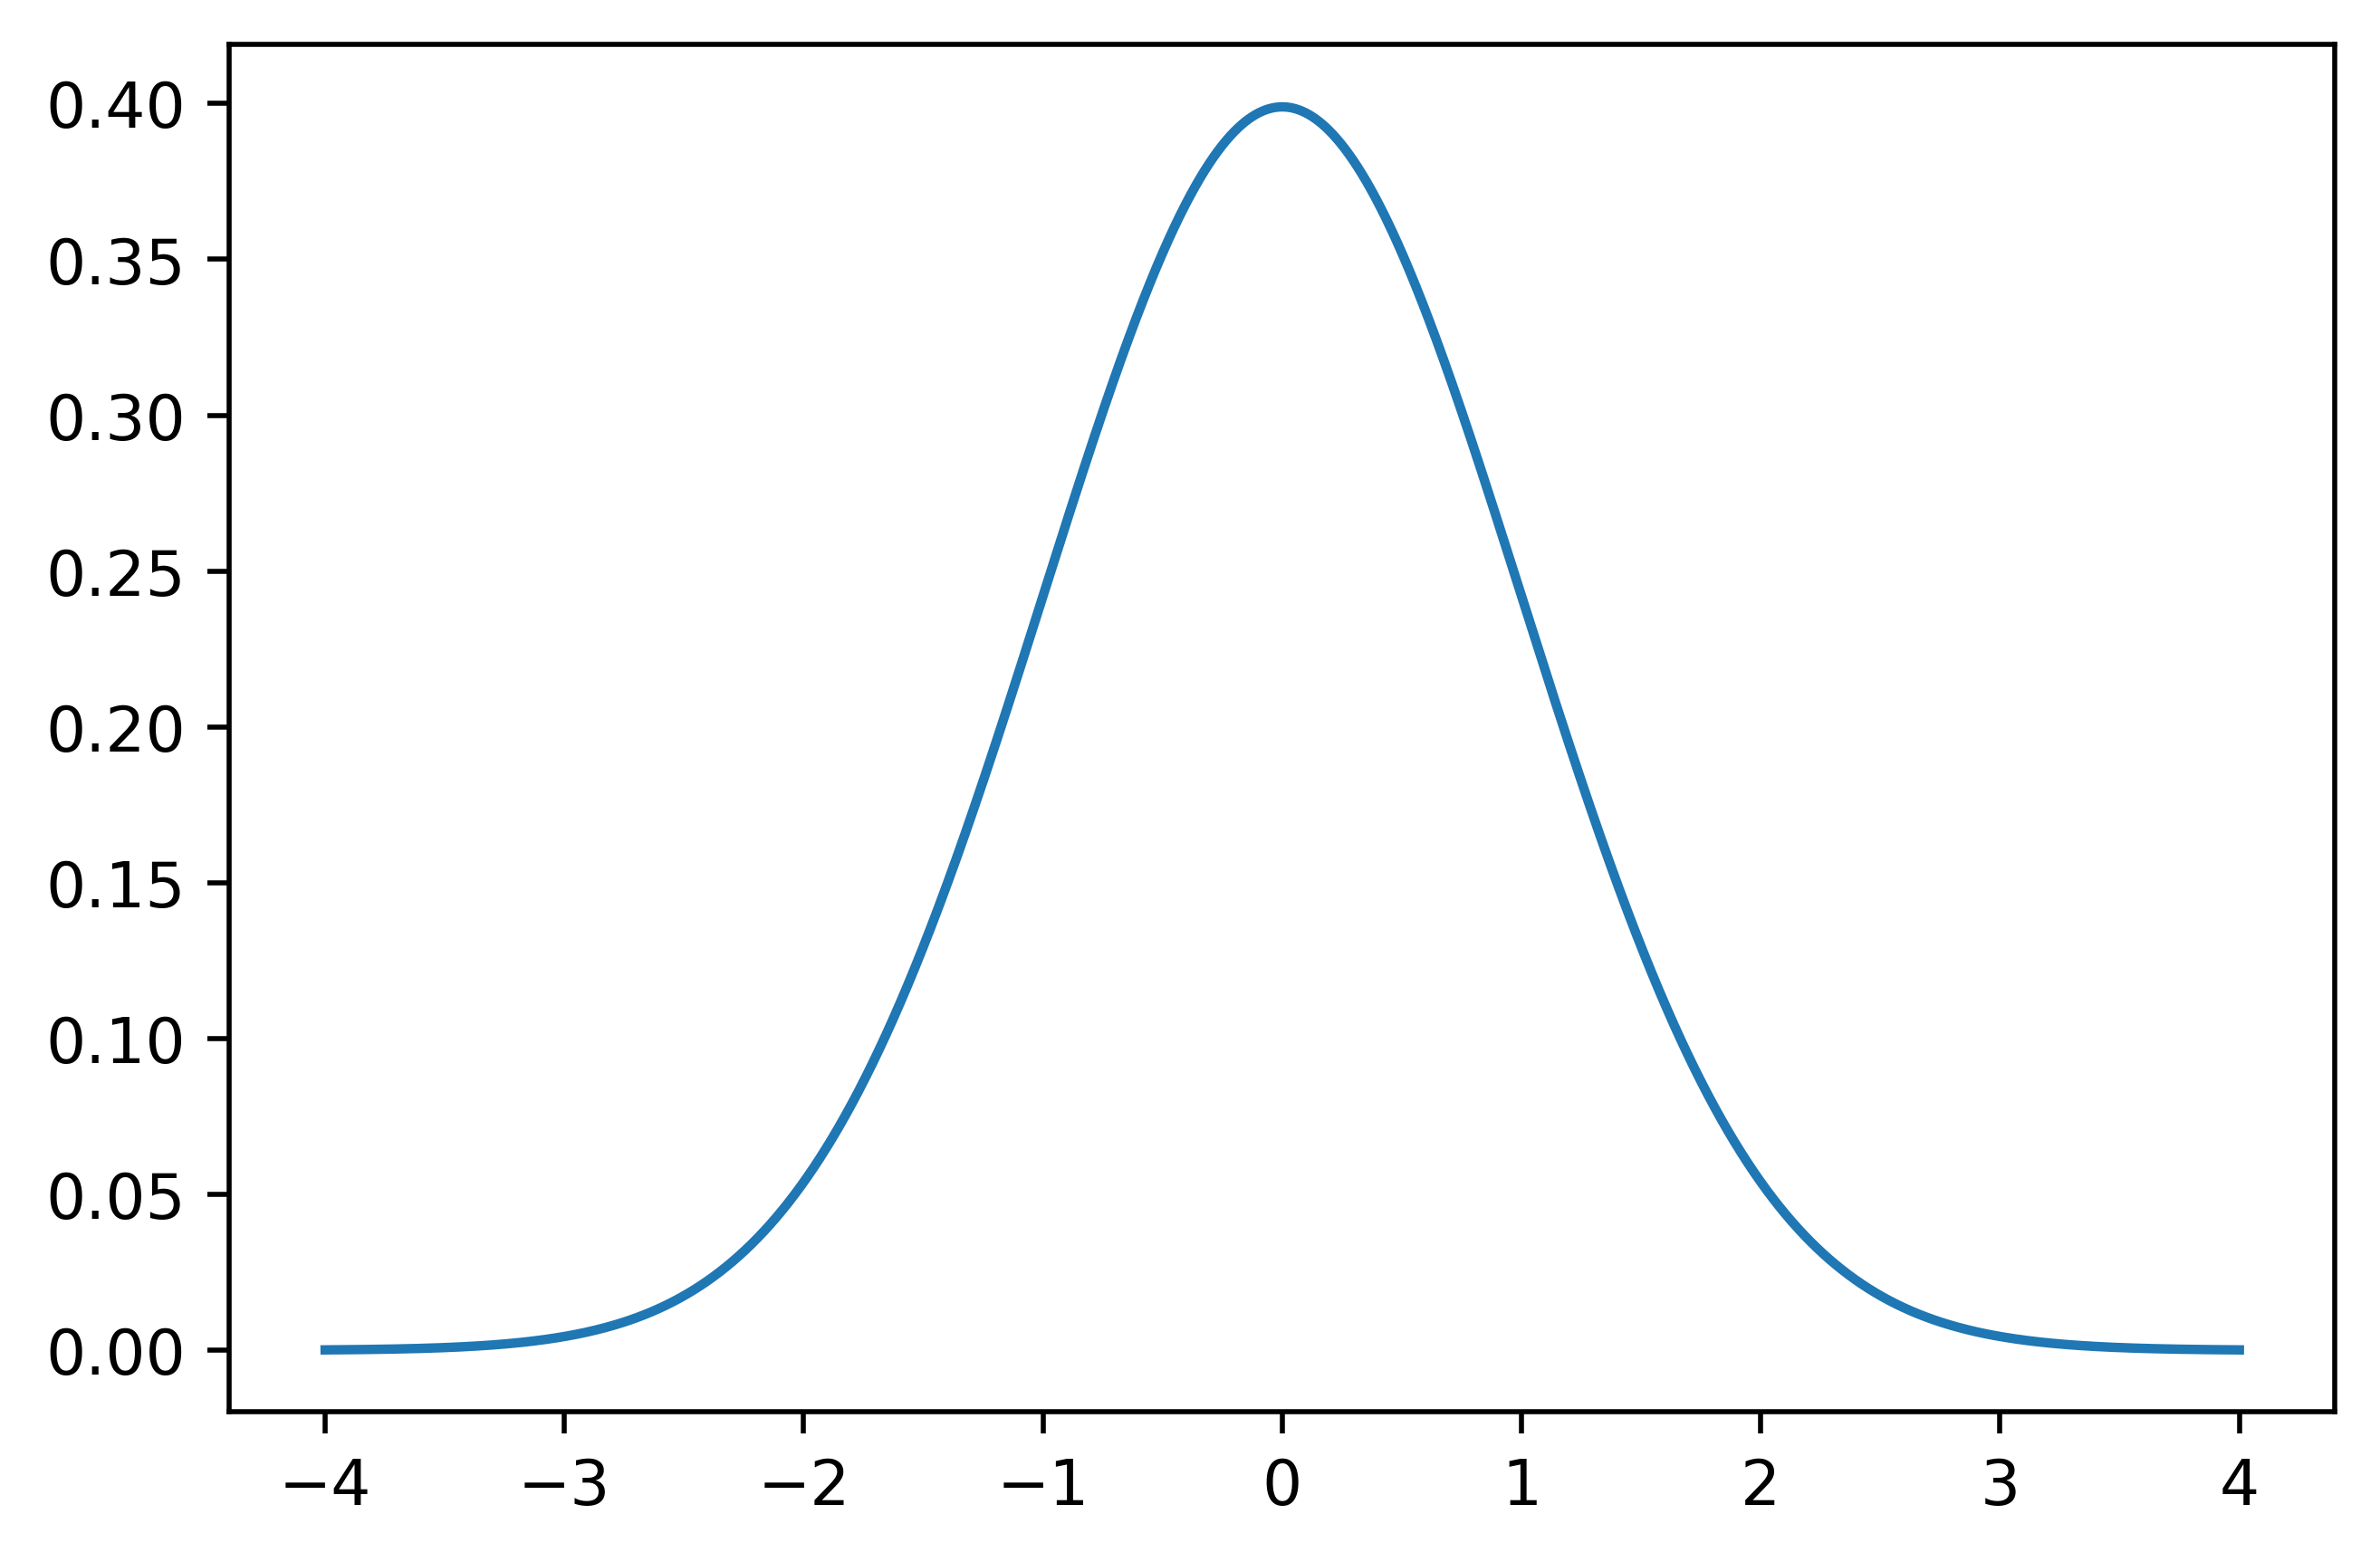
\includegraphics[scale=0.5]{images/gaussian.png}
        \caption{PDF of standard normal distribution}
        \label{normal_pdf}
    \end{figure}
    \item \textbf{Continuous uniform distribution}: Here, we have used U(0, 1). The PMF is given by $$f_X(x) = \begin{cases}1,\; 0 \le x \le 1 \\ 0,\; otherwise\end{cases}$$ 
    The mean is 0.5 and standard deviation is 0.289. Figure \ref{uni_pdf} shows the PDF of the uniform distribution.
    \begin{figure}[H]
        \centering
        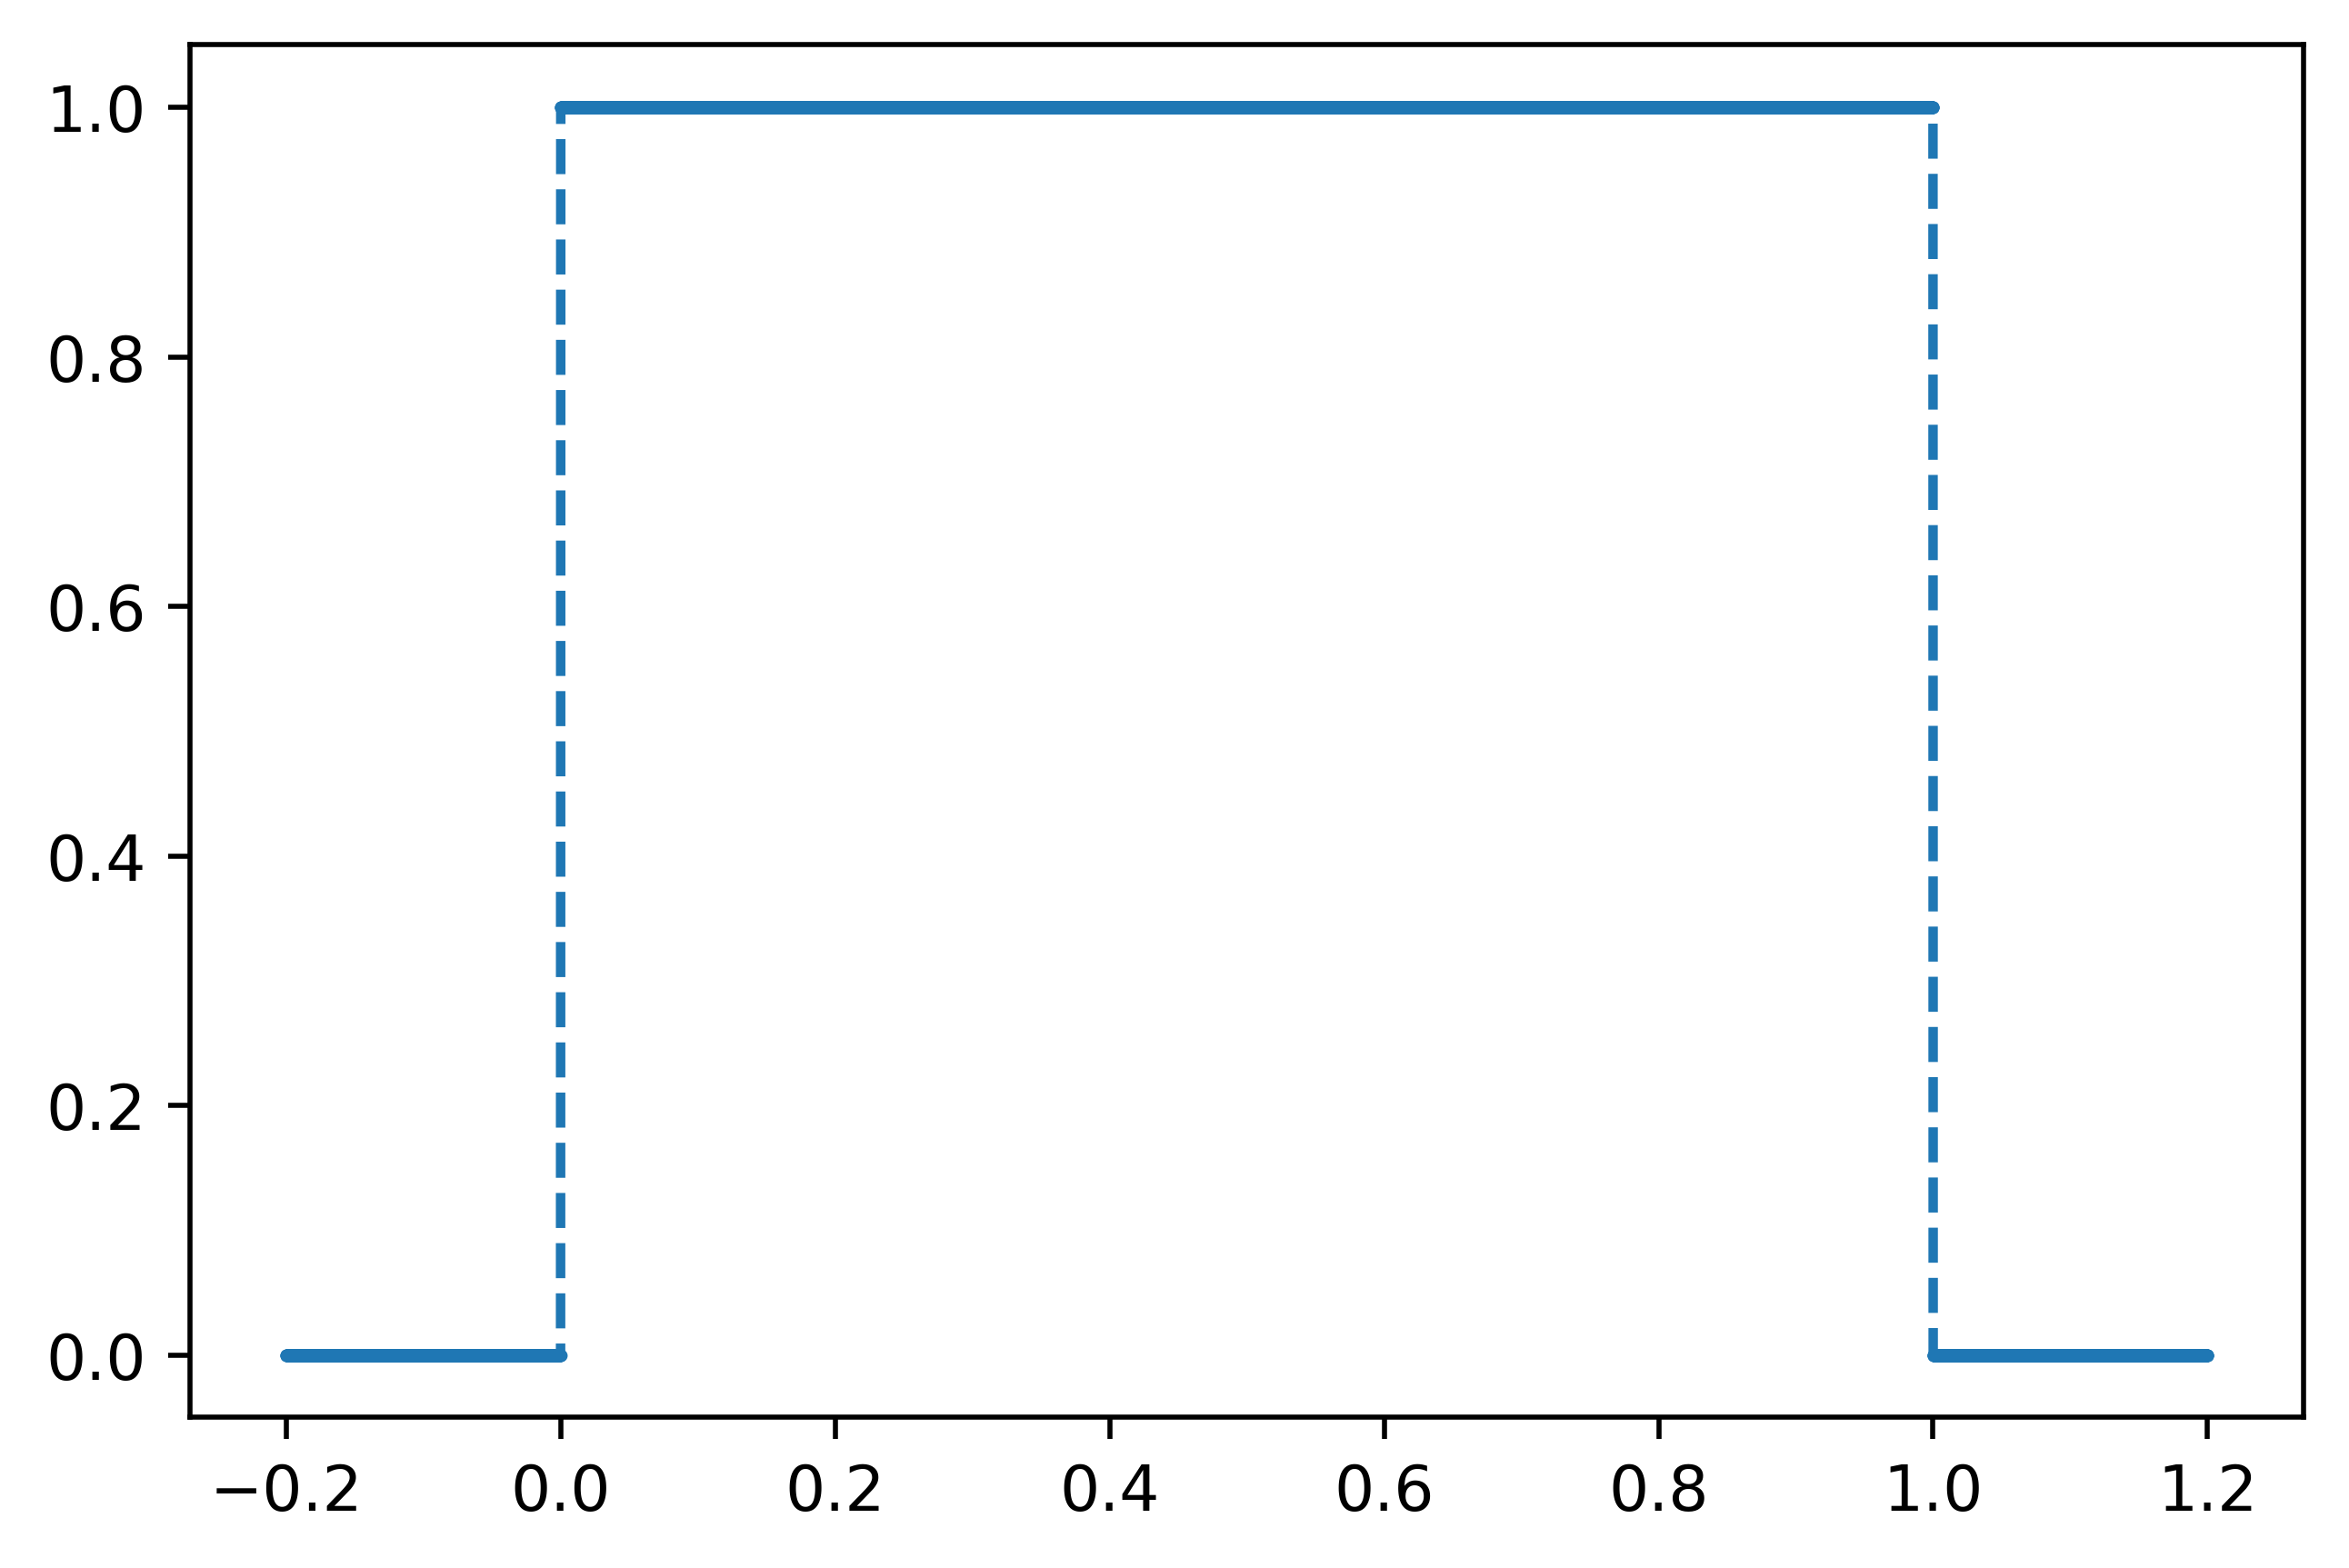
\includegraphics[scale=0.5]{images/uniform.png}
        \caption{PDF of uniform distribution}
        \label{uni_pdf}
    \end{figure}
    \item \textbf{Geometric Distribution}: Unlike the other distributions that we used, this distribution is for a discrete random variable. The PMF is given by
    $$f_X(k) = (1-p)^{k-1}p,\; k=1,2,3,...$$
    In our experiments, we arbitrarily chose to use $p=0.35$. The mean is $\dfrac{1}{p}$ and the standard deviation is $\dfrac{\sqrt{1-p}}{p}$. The PMF is given in figure \ref{geom_pmf}. 
    \begin{figure}[H]
        \centering
        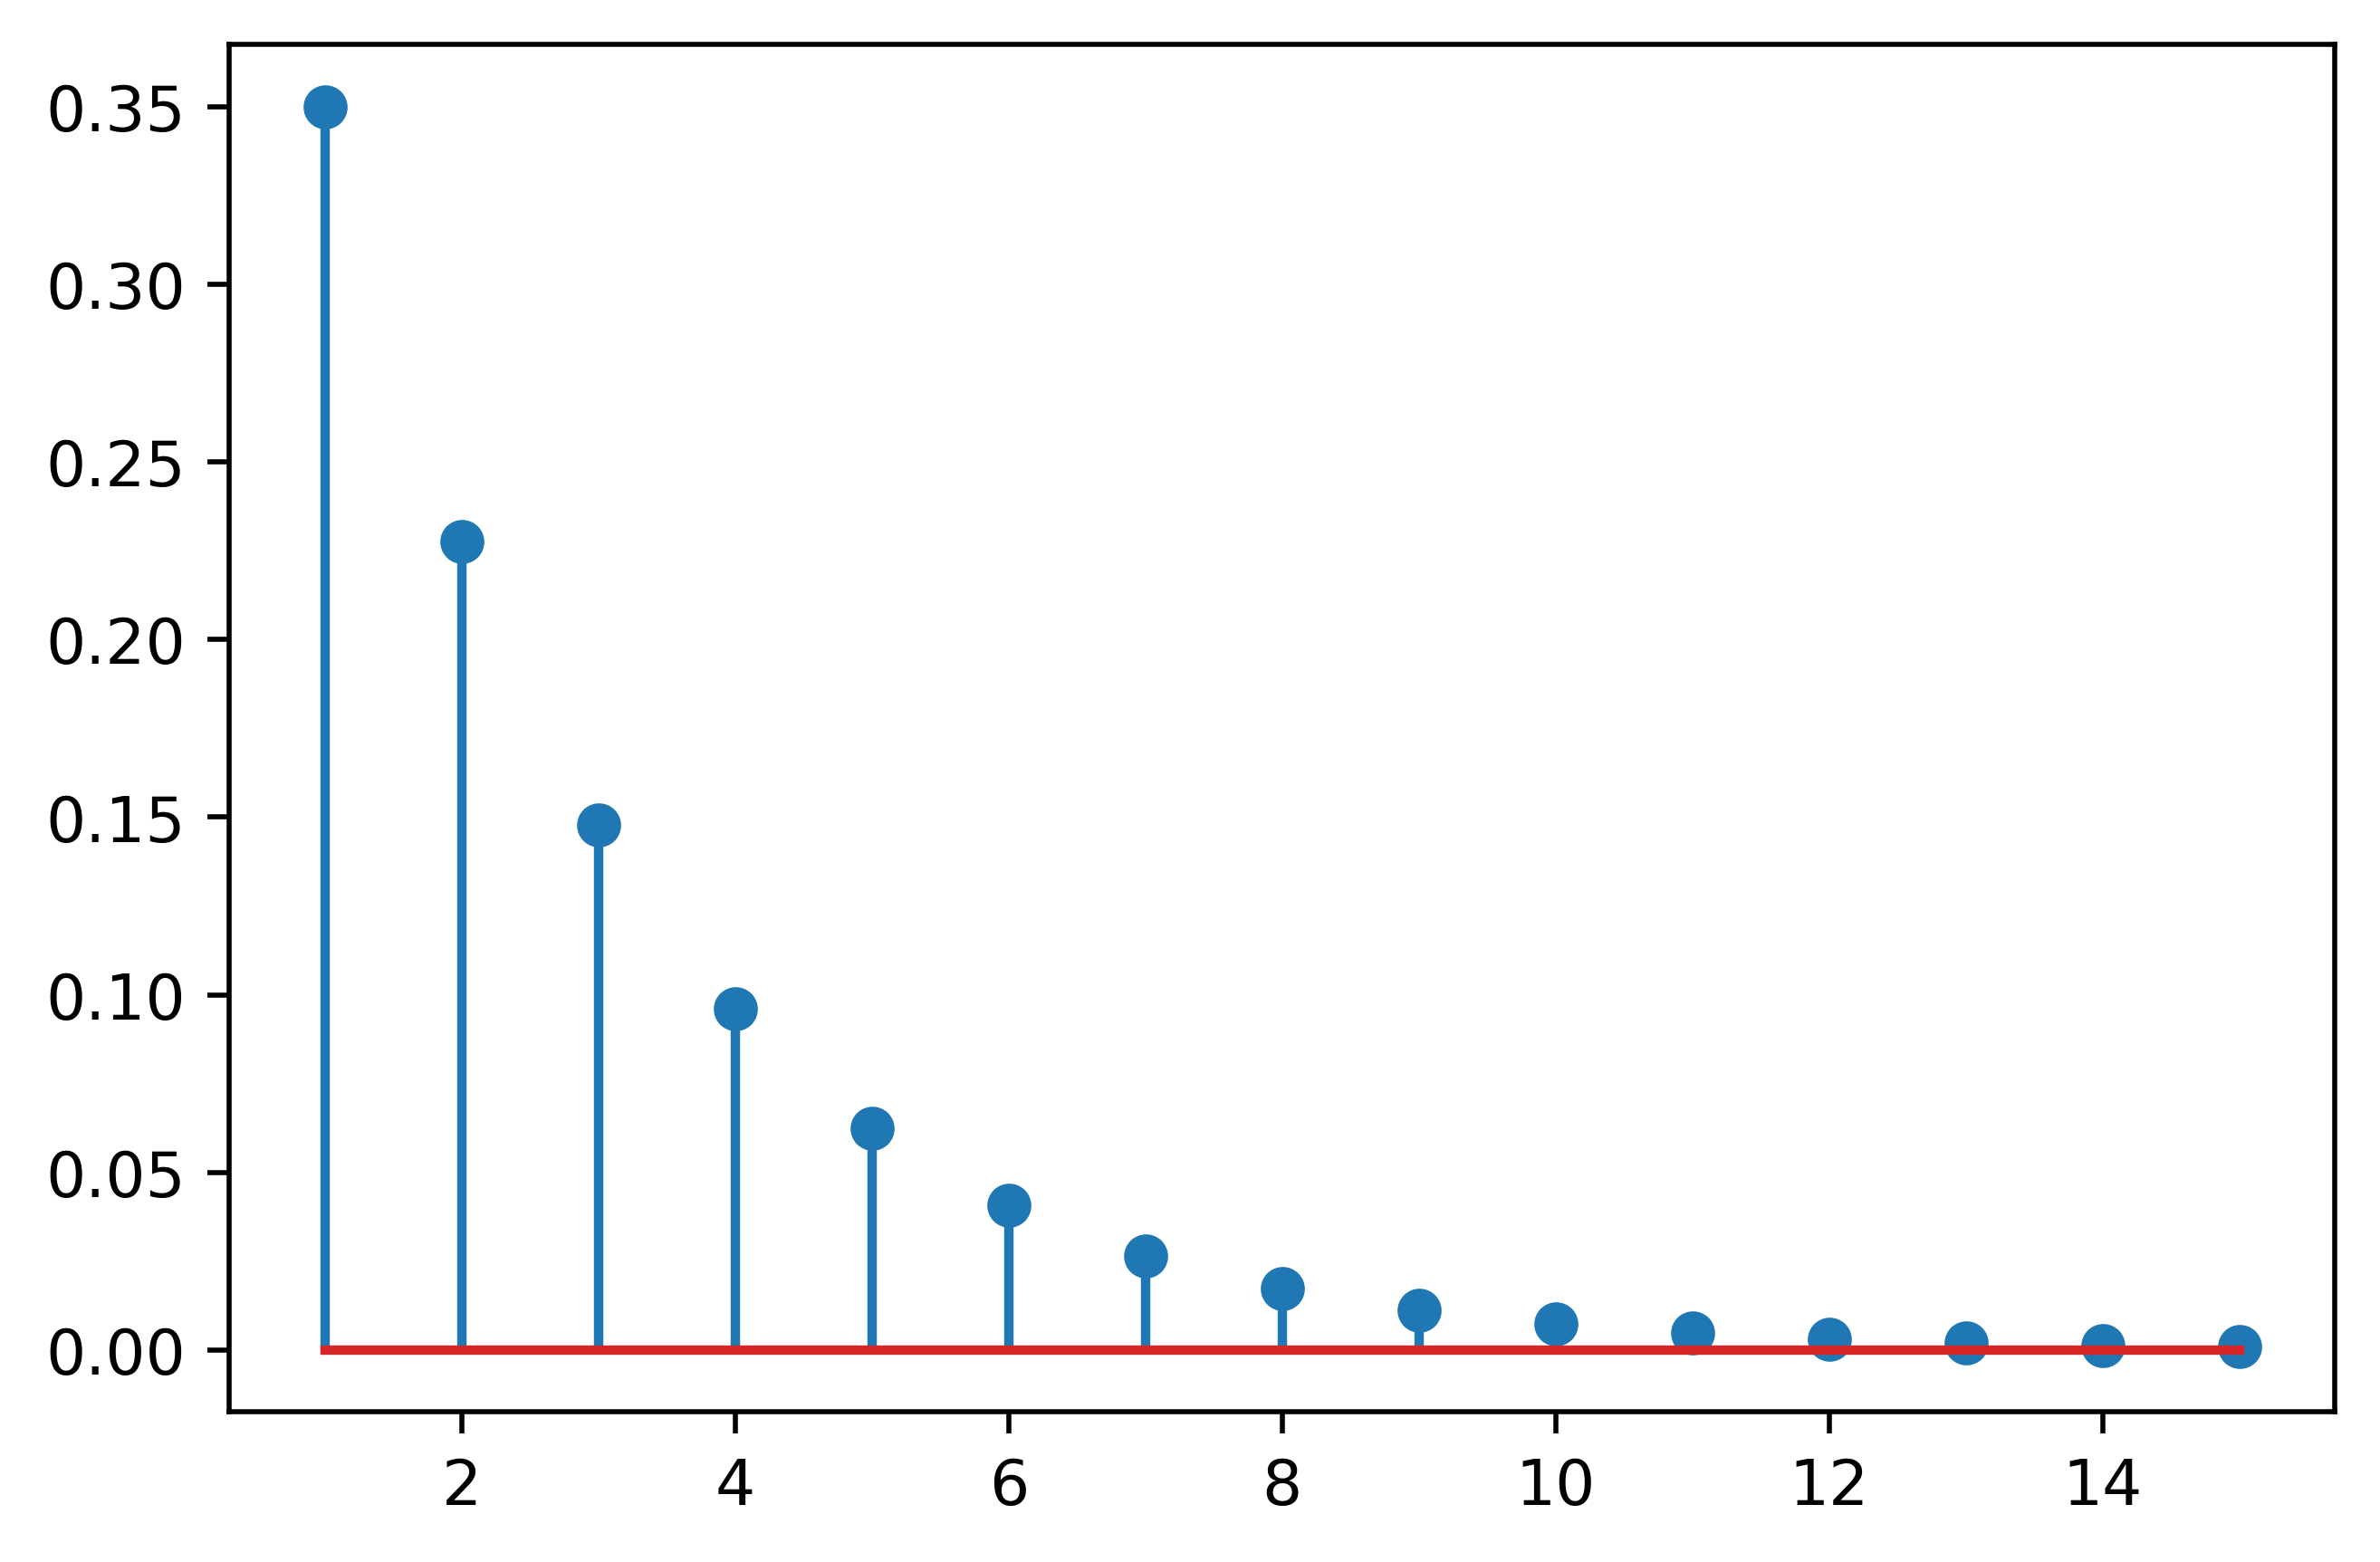
\includegraphics[scale=0.5]{images/geometric.png}
        \caption{PMF of geometric distribution}
        \label{geom_pmf}
    \end{figure}
    \item \textbf{Standard cauchy distribution}: The PDF is given by $$f_X(x) = \dfrac{1}{\pi (1+x^2)}$$ Neither the mean nor the standard deviation are finite. Thus CLT should not apply on this distribution. Figure \ref{cauchy_pdf} shows the PDF of standard cauchy distribution.
    \begin{figure}[H]
        \centering
        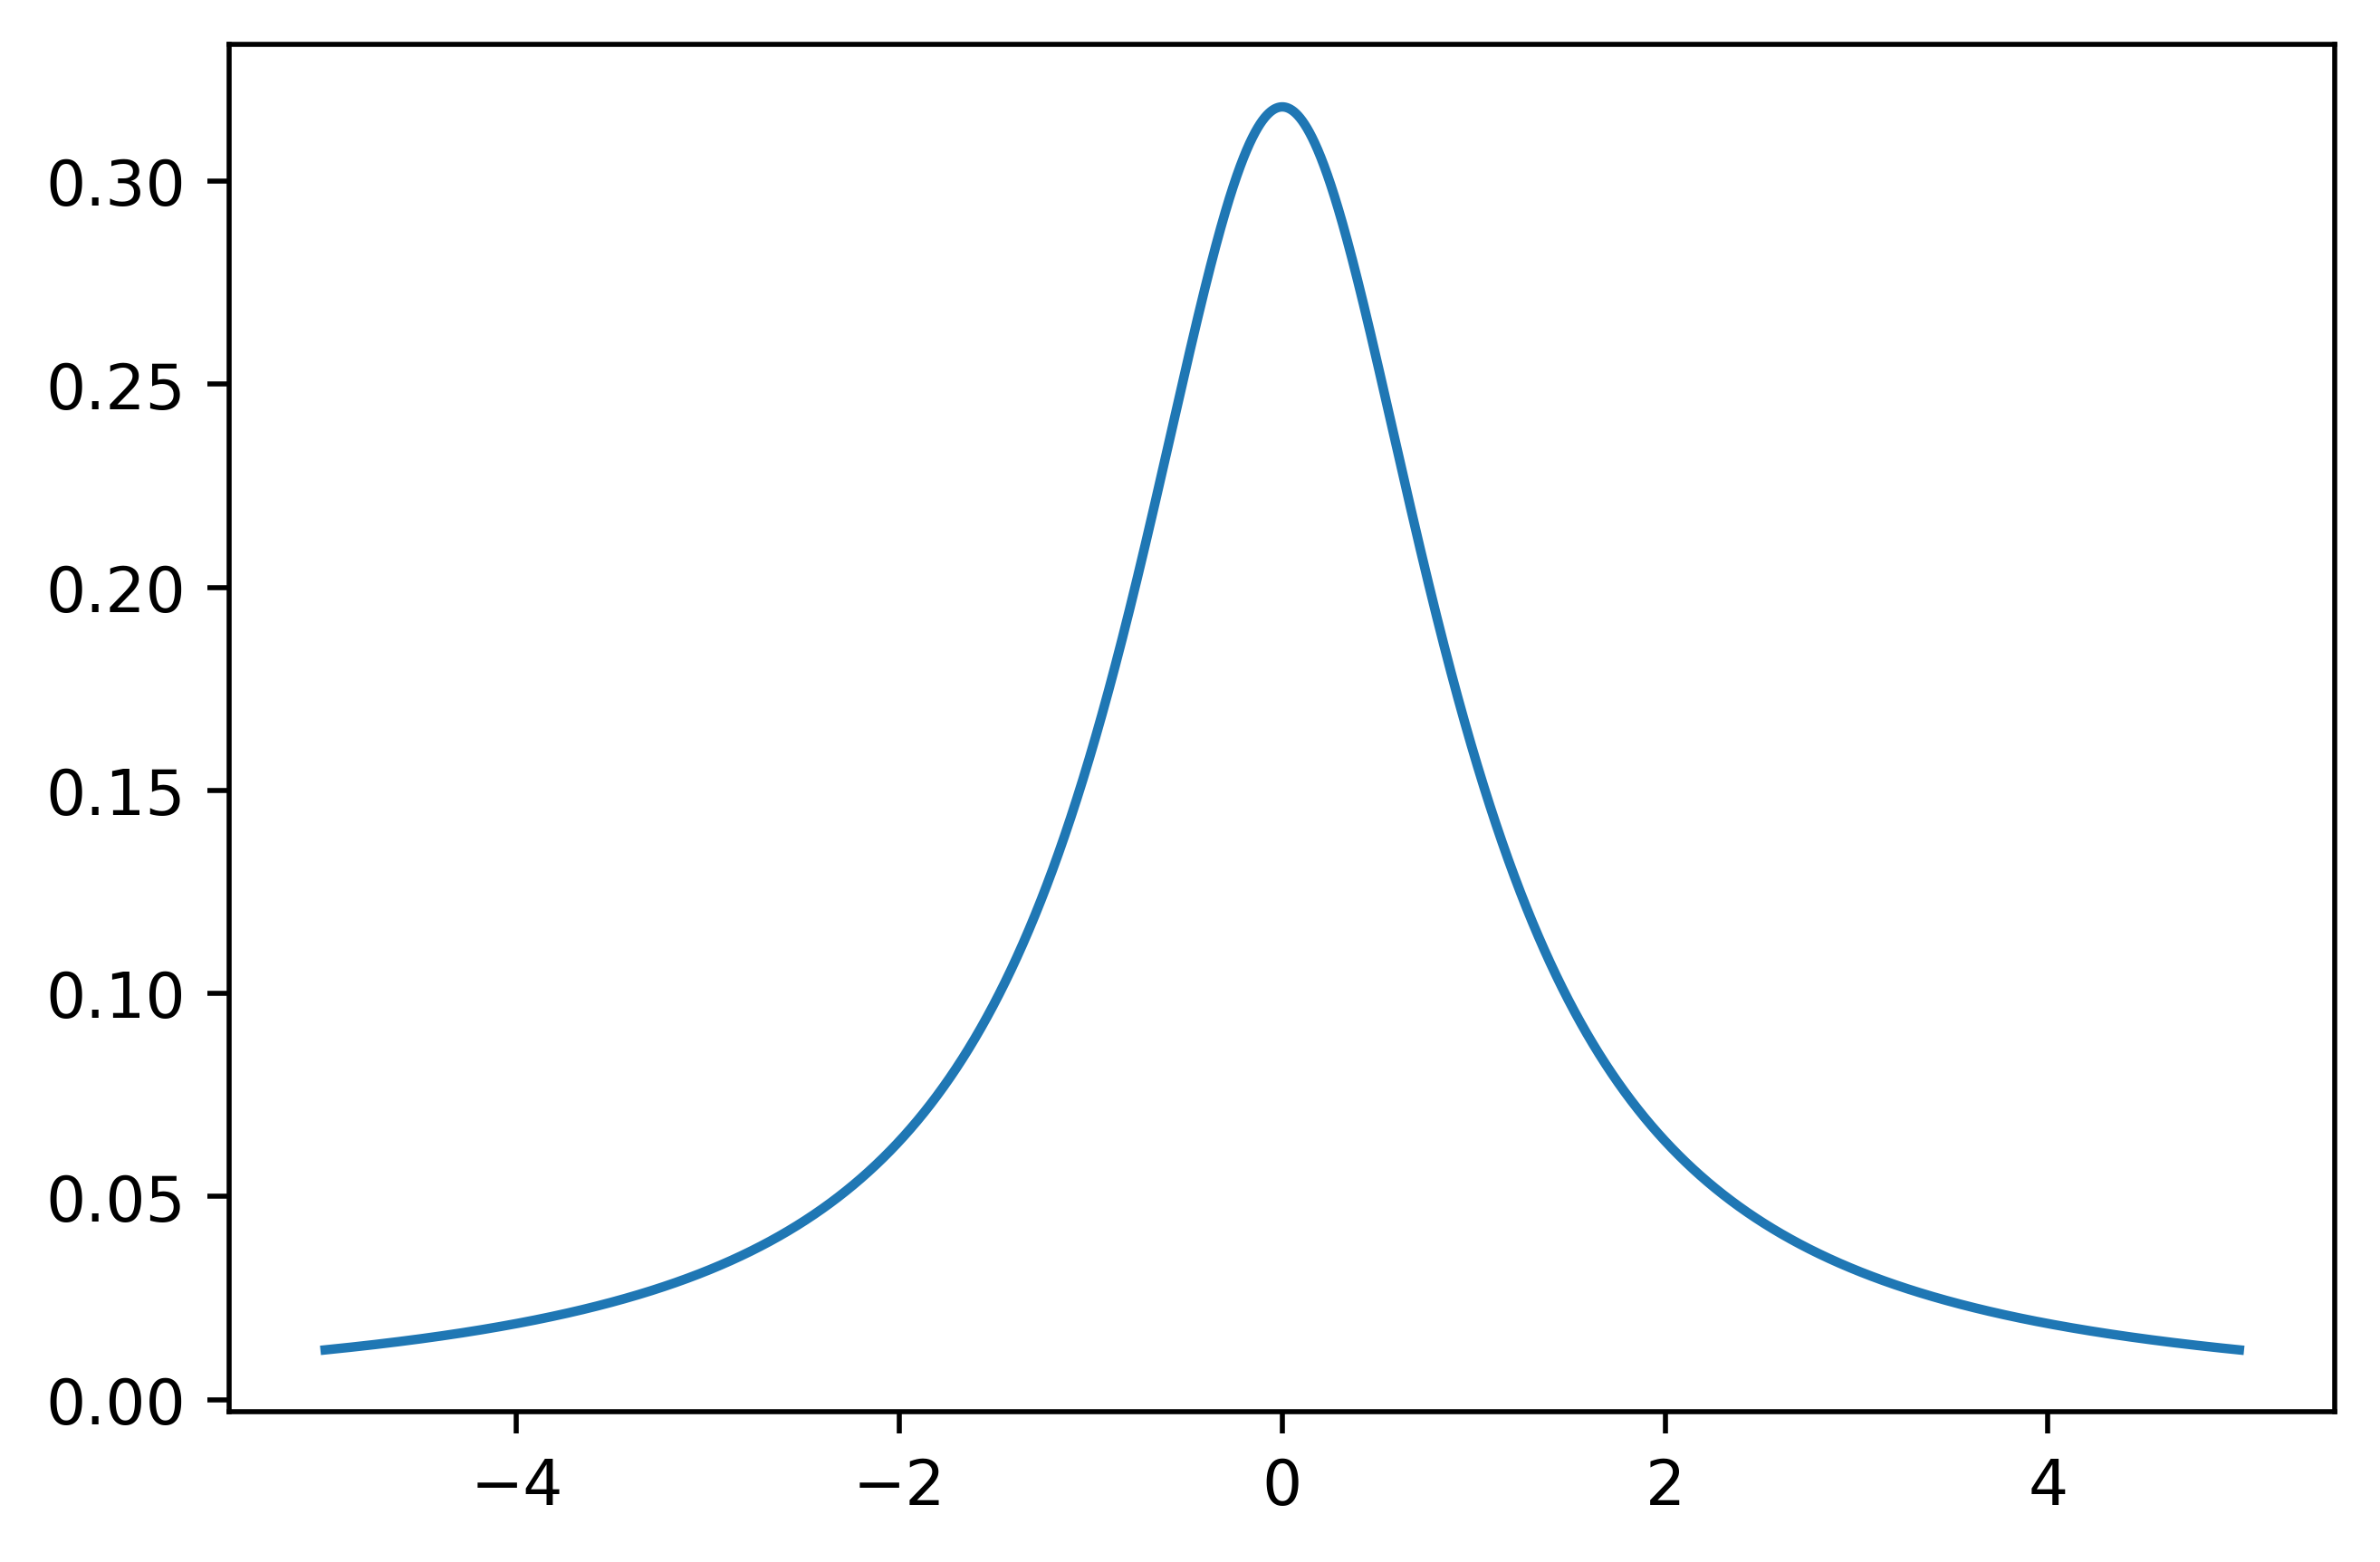
\includegraphics[scale=0.4]{images/cauchy.png}
        \caption{PDF of Cauchy Distribution}
        \label{cauchy_pdf}
    \end{figure}
\end{enumerate}
The code used for generating images of these distribution can be found \href{https://github.com/cmaspi/verifying_CLT/blob/main/codes/distribution_images.ipynb}{here}

\section{Results}
For Normal distribution and uniform distribution, we found that even for the smallest selected sample size of 10, the sample mean follows Normal distribution as per Shapiro-Wilk test. Thus CLT holds true for these for any sample size greater than or equal to 10. For Geometric distribution, we found that CLT did not hold for sample sizes 10 and 30 as per Shapiro-Wilk test. However, CLT held true for sample sizes 50 and 100. For Cauchy distribution, we found that CLT did not hold for any sample size. 

\noindent You can find the python codes for the above results 
\href{https://github.com/cmaspi/verifying_CLT/blob/main/codes/visualise_hist.ipynb}{here}.

\section{Conclusion}
While using CLT, the empirical approximation is a good one but it may fail. To get better results, one may want to consider using a larger sample size of 50. Also, one may want to verify that the sampling distribution has finite mean and sample variance before applying CLT.

\section{Source Repository}
The repository containing all codes, latex files, images can be found \href{https://github.com/cmaspi/verifying_CLT}{here}

\section{References}
\begin{enumerate}
    \item Wikipedia contributors. \href{https://en.wikipedia.org/wiki/Central_limit_theorem}{Central Limit Theorem}
    \item Wikipedia contributors. \href{https://en.wikipedia.org/wiki/Shapiro\%E2\%80\%93Wilk_test}{Shapiro-Wilk test}
    \item Wikipedia contributors \href{https://en.wikipedia.org/wiki/Cauchy_distribution}{Cauchy Distribution}
    \item link-springer. \href{https://link.springer.com/content/pdf/bbm\%3A978-1-4684-0167-7\%2F1.pdf}{Shapiro-Wilk test (pdf)}
    \item \href{https://math.mit.edu/~rmd/465/shapiro.pdf}{Shapiro-Wilk test and related tests for normality (pdf)}
\end{enumerate}

\section{Contribution}
\begin{itemize}
    \item Chirag: Sections 1, 4, 5 and Code (distribution\_images.ipynb and part of visualise\_hist.ipynb)
    \item Dishank: Sections 5, 6, 7 and Code(visualise\_hist.ipynb)
    \item Savarana Datta: Section 3, Slides and Code (example.ipynb)
    \item Vishwanath: Section 2 and Slides
\end{itemize}

\end{document}
